\normaltrue \difficilefalse \tdifficilefalse
\correctionfalse

%\UPSTIidClasse{11} % 11 sup, 12 spé
%\newcommand{\UPSTIidClasse}{12}

\exer{Train simple $\star$ \label{C2:06:37}}
\textit{D'après ressources Pole Chateaubriand -- Joliot-Curie.}
\setcounter{question}{0}\UPSTIcompetence[2]{A3-05}
\UPSTIcompetence[2]{C2-06}
\index{Compétence C2-06}
%\index{Train d'engrenages simple}
\ifcorrection
\else
\marginnote{\textbf{Pas de corrigé pour cet exercice.}}
\fi

\ifprof
\else
L’usinage est une opération de transformation d’un produit par enlèvement de matière.
Cette opération est à la base de la fabrication de produits dans les industries mécaniques.
La génération d’une surface par enlèvement de matière est obtenue grâce à un outil muni
d’au moins une arête coupante. Les différentes formes de pièces sont obtenues par des
translations et des rotations de l'outil par rapport à la pièce.


On s’intéresse ici à l’axe Y qui met en mouvement le coulisseau 1,
sur lequel est fixée l’outil, par rapport au bâti 0. Le coulisseau 1 est mis en mouvement par un moteur
électrique qui délivre un couple moteur $C_m(t)$.

\begin{center}
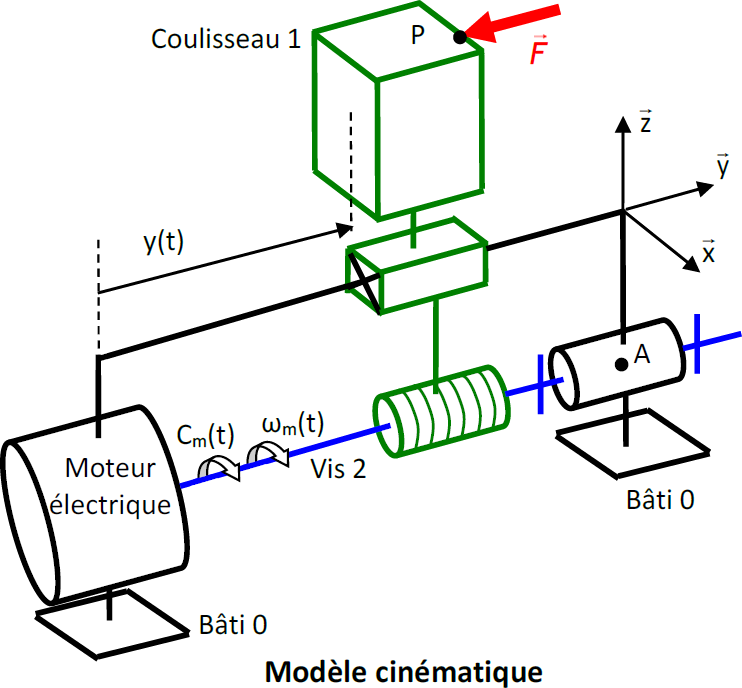
\includegraphics[width=\linewidth]{37_01}
\end{center}

On note $p$ le pas de vis. 
\fi


\question{Tracer le graphe des liaisons.}
\ifprof
\else
\fi

\question{Définir la loi entrée-sortie entre la vitesse de translation du coulisseau et la vitesse de rotation du moteur.}
\ifprof ~\\
\else
\fi

\ifprof
\else
\begin{flushright}
\footnotesize{Corrigé  voir \ref{C2:06:37}.}
\end{flushright}%
\fi